\begin{figure}[htbp]
  \centering
  \begin{subfigure}{.16\textwidth}
    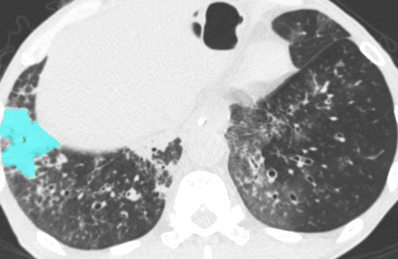
\includegraphics[width=1\linewidth]{images/examples/consolidation.png}
    \caption{CON \textcolor{cyan}{$\blacksquare$}} \label{fig:example_con}
  \end{subfigure}
  \qquad
  \begin{subfigure}{.16\textwidth}
    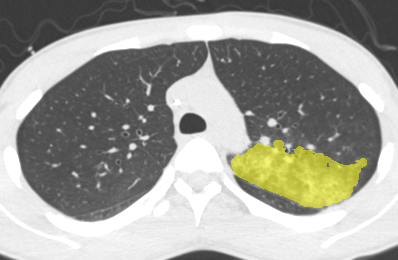
\includegraphics[width=1\linewidth]{images/examples/ggo.png}
    \caption{GGO \textcolor{yellow}{$\blacksquare$}}
  \end{subfigure}
  \qquad
  \begin{subfigure}{.16\textwidth}
    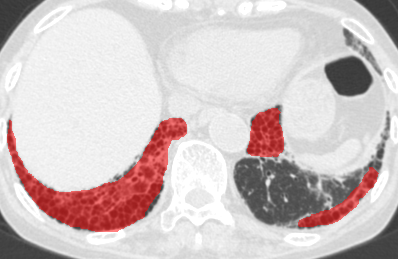
\includegraphics[width=1\linewidth]{images/examples/hcm.png}
    \caption{HCM \textcolor{red}{$\blacksquare$}}
  \end{subfigure}
  \qquad
  \begin{subfigure}{.16\textwidth}
    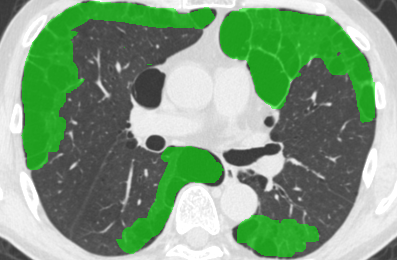
\includegraphics[width=1\linewidth]{images/examples/emp.png}
    \caption{EMP \textcolor{green}{$\blacksquare$}}
  \end{subfigure}
  \qquad
  \begin{subfigure}{.16\textwidth}
    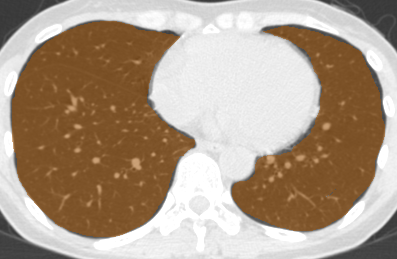
\includegraphics[width=1\linewidth]{images/examples/nor.png}
    \caption{NOR \textcolor{brown}{$\blacksquare$}}
  \end{subfigure}
  \caption{Typical slices for each DLD classes.
    Slices of HRCT are shown in  lung window setting (window-center=-600, window-width=1500) with annotated labels superimposed in transparent colors.
    Note that even if more than one DLD patterns existed, only one DLD pattern was chosen and annotated for a slice to facilitate the annotation process.}
  \label{image_examples}
\end{figure}
